% !TEX root = twe2.tex

\section{Literatur}
\label{sec:Literatur}

Aufgrund der preiswerten Versorgung von Proteinen über importiertes Soja ist die N-Quelle Leguminosen für Milchkuhhalter bisher kaum erschlossen.
Inzwischen verlangen aber immer mehr Verbraucher Produkte welche unter Gesichtspunkten des Umweltschutzes und Ressourcenschonung produziert wurden.
Dadurch ist der Einsatz von importierten Soja für einige Betriebe nicht mehr möglich bzw. erschwert die Vermarktung der Milch und diese Milcherzeuger müssen daher andere Proteinquellen erschließen.

\subsection{Einfluss auf \acl{TM}-Erträge}
\label{subsec:TM}

Die Grasbestände sind insbesondere auf einen hohen \ac{TM}-Ertag ausgelegt.
Dieser wird über sehr ertragsreiche, aber auch auf N-Düngung angewiesenen Arten und Sorten erreicht.
Allerdings hat sich bereits gezeigt, dass eine Artenreiche Gräsermischung, insbesondere mit Leguminosen, höhere Erträge liefern können als Reinsaaten der ertragreichsten Art \parencite{nyfeler2009strong}.\todo{Seitenzahl einfügen!}
Leguminosen reduzieren die N\textsubscript{2}-Fixierung bei N-Düngung \parencite{ledgard2001nitrogen}\todo{Seitenzahl einfügen}, weswegen die N-Düngung zumindestens reduziert werden muss \parencite[34]{weggler2050leguminosen}.

Bei einer Reduzierung der N-Düngung, um die Leguminosen in den Bestand zu integrieren, besteht die Möglichkeit, dass die \ac{TM}-Erträge absinken könnten.
Dies ist zu vermeiden, da viele Betriebe darauf angewiesen sind, mit den vorhanden Flächen ausreichend Futter für Ihre Tiere zu produzieren.
Nach \textcite[11]{engel2013protein} sind die Verluste an \ac{TM}-Ertrag bei einer Reduzierung der N-Düngung von 240\,kg\,N\,ha\textsuperscript{-1}a\textsuperscript{-1} ohne Leguminosen auf 80\,kg\,N\,ha\textsuperscript{-1}a\textsuperscript{-1} mit Weißklee bei etwa 20\%.

Allerdings ist auch zu erwähnen, dass die \ac{EU} eine Düngung von 240\,kg\,N\,ha\textsuperscript{-1}a\textsuperscript{-1} eventuell, im Zuge der gemeinsamen Agrarpolitik oder indirekt über andere Vorgaben, verboten oder eingeschränkt könnte.
Daher scheint der Vergleich von 160\,kg\,N\,ha\textsuperscript{-1}a\textsuperscript{-1} ohne Leguminosen mit 80\,kg\,N\,ha\textsuperscript{-1}a\textsuperscript{-1} mit einem Leguminosenanteil unter langfristigen Gesichtspunkten verständlich.
Da betriebseigener Wirtschaftsdünger i.d.R. kostengünstig zur Verfügung steht, ist eine gewisse N-Düngung wirtschaftlich nur schwer komplett zu vermeiden.
In diesem Fall reduziert sich der \ac{TM}-Ertrag nach \textcite[11]{engel2013protein} um etwa 2,5\%.
Leider sind keine Konfidenzintervalle angegeben, sodass eine Aussage über die statistische Signifikanz hier leider nicht möglich ist.
Allerdings ist eine Abweichung von 2,5\% auch relativ gering und wird in der Praxis wohl auch kaum bemerkt werden.

Der positive Einfluss von Rotklee auf den \ac{TM}-Ertrag wurde von \textcite[242]{FrankowLindberg2009} gezeigt und wird von den Ergebnissen von \textcite[35]{weggler2050leguminosen} gestützt.
In \cref{fig:wegglerAbb1} ist zu erkennen, dass der \ac{NEL}-Ertrag bei eienr Rotkleenachsaat steigt während der \ac{NEL}-Gehalt des Futtermittels sinkt.
Dies ist nur duch einen starken positiven Effekt auf den \ac{TM}-Ertrag zu erklären.


%Nach \textcite[35-36]{weggler2050leguminosen} sind die \ac{NEL} Erträge je Hektar bei Rotklee größer als bei Weißklee, allerdings sinkt bei der Rotkleevariante der \ac{NEL}-Gehalt des Aufwuchses.
%Dies bedeutet, dass mit einer Rotkleenachsaat nicht nur der \ac{NEL} Ertrag gesteigert werden kann, sondern auch der \ac{TM} Ertrag.
%Allerdings geht dies zu Lasten des \ac{NEL}- und \ac{XP}-Gehalts welches den Futterwert deutlich senkt.
%Da die Futteraufnahme der Tiere begrenzt ist, ist mit einem Rückgang der Milchleistung aus dem Grundfutter zu rechnen.

\subsection{Einfluss auf den \acl{XP}-Etrag}
\label{subsec:Protein}

Auch wenn Leguminosen generell die Möglichkeit haben hohe \ac{XP}-Gehalte \todo{Zitat} zu generieren, stellt sich die Frage ob eine Nachsaat von Leguminosen ausreicht um die \ac{XP}-Gehalte bei einer Reduizierung der N-Düngung zu erhöhen oder wenigstens konstant zu halten.
Nach \textcite[11]{engel2013protein} ist es bei reduzierter N-Düngung möglich unter bestimmten Bedingungen die \ac{XP}-Gehalte leicht zu steigern.
Natürlich hängen die \ac{XP}-Erträge und -Gehalte von vielen Faktoren ab, daher müssen insbesondere geringe Unterschiede genau betrachtet werden.
Eine genauere Untersuchung von \textcite{weggler2020langzeitbeobachtungen} hat gezeigt, dass die \ac{XP}-Erträge bei \todo{nachlesen!!!}  moderater N-Düngung (ca. 150\,kg\,N\,ha\textsuperscript{-1}) im dreijährigen Mittel gesteigert werden konnten.
Bei einer Rotkleenachsaat waren eine signifikante Steigerung des \ac{XP}-Ertrages von etwa\todo{kurze Abstände zwischen Einheiten okay?} 3\,dt\,ha\textsuperscript{-1}a\textsuperscript{-1} möglich \parencite[12]{weggler2020langzeitbeobachtungen}, allerdings konnte der \ac{XP}-Gehalt nur in Einzelfällen gesteigert werden \parencite[13]{weggler2020langzeitbeobachtungen}.


Die N-Düngung von Flächen, auf welchen zuvor Leguminosen nachgesäät wurden, hatte nach \textcite[34]{weggler2050leguminosen} keinen signifkanten Einfluss auf den \ac{XP}-Gehalt.
Allerdings profitieren Gräser von einer hohen N-Düngung und verdrängen somit sowohl Weiß- als auch Rotklee aus dem Bestand \parencite[161]{black2009clover}.


\begin{figure}
	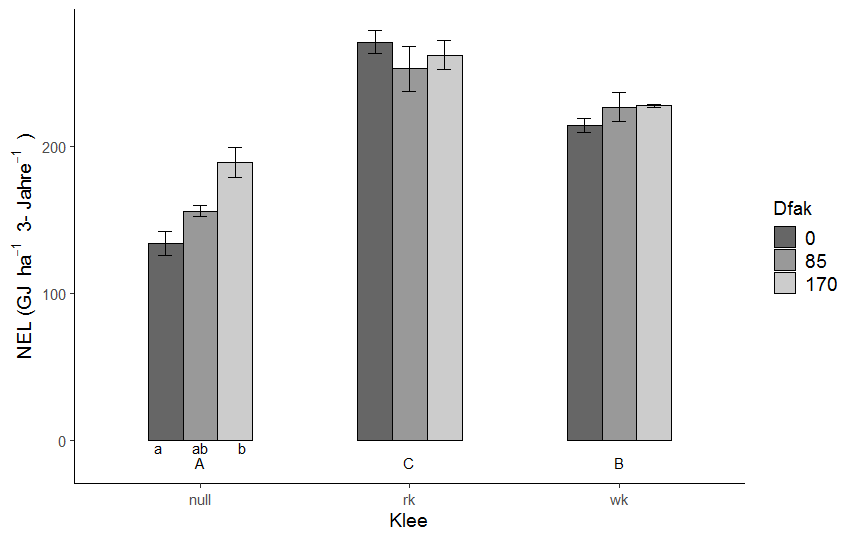
\includegraphics[scale=0.5]{images/wegglerAbb2}
	\caption[\ac{NEL}-Erträge der verschiedenen Varianten über 3 Jahre aufsummiert]{\ac{NEL}-Ertäge der verschiedenen Varianten über 3 Jahre aufsummiert \parencite[36]{weggler2050leguminosen}}
	\label{fig:wegglerAbb2}
\end{figure}

\subsection{Einfluss auf den \acl{NEL}-Ertrag}
\label{subsec:NEL}
Die Untersuchung von \textcite{weggler2050leguminosen} auf den Einfluss von Klee auf den \ac{NEL}-Ertrag ist eine der ersten Arbeiten mit dieser Zielsetzung.
Es wird gezeigt, dass die \ac{NEL}-Erträge bei einer Rotkleenachsaat gesteigert werden können, während der \ac{NEL}-Gehalt sinkt, wobei beide Effekte statistisch signifikant waren.
Die Steigerung des \ac{NEL}-Etrags durch die Rotkleenachsaat war bei einer N-Düngung von 170\,kg\,N\,ha\textsuperscript{-1}a\textsuperscript{-1} etwa 55\% (siehe \cref{fig:wegglerAbb2}).
Eine Weißkleenachsaat hat mit einer Steigerung von 16\% einen deutlich geringeren Effekt auf den \ac{NEL}-Ertrag.
Dafür waren durch die Weißkleenachsaat die \ac{NEL}-Gehalte weiterhin auf einem ähnlichen Niveau.
%Generell setzen Pflanzen N in \ac{XP} um, um über die Chloroplasten Photosynthese betreiben zu können.
%Daher ist eine ausreichende N-Versorgung essentiell für hohe Erträge.\todo{Hier ist noch ein bisschen was zu schreiben, evtl noch ein bisschen was zu lesen}


\subsection{Stickstoffbedarf der Milchproduktion}
\label{subsec:Stickstoff}
Betriebe sind aufgrund der \ac{DUV} verpflichtet über, z.B. die Hoftorbilanz, die N-Bilanz des Betriebes zu berechnen.
Viele Betriebe haben dabei positive Saldi \parencite[7ff.]{lellmann2005untersuchungen} und müssen daher weitere N-Quellen meiden.
Eine große, und in den meisten Fällen außerbetrieblieche Quelle, ist das Kraftfutter \parencite[62]{lellmann2005untersuchungen}.

Stickstoffverluste treten insbesondere über den Verkauf von Milch über das Milcheiweiß auf. \todo{Zitat}
Zum anderen entstehen beim Wirtschaftsdünger unvermeidbare N-Verluste bei der Lagerung und Ausbringung.\todo{cite lellmann?}
Deweiteren entstehen auf den Feldern, insbesondere bei hoher N-Düngung, Nitratauswaschungen.
Diese stehen immer stärker in der Kritik, da diese das Grundwasser erreichen können und Nitrat im Körper zum Nitrit umgewandelt wird.
Da Nitrit giftig ist, hat die \ac{EU} einen strengen Grenzwert von 50\,mg\,l\textsuperscript{-1} Nitrat im Grundwasser festgelegt.\todo{Zitat}
Da Deutschland den Grenzwert von Nitrat im Grundwasser nicht einhalten kann, wird über die \ac{DUV} das Ziel verfolgt, den Grundwasserkörper zu verbessern.


\subsection{Ernteverluste}
\label{subsec:Lit:Ernte}

%Nachdem die \ac{XP} erfolgreich auf dem Feld produziert wurden, müssen diese konserviert werden.
Eine erfolgreiche Konservierung des Grünlandaufwuchses ist wichtig.
Da ein großerTeil des Grünlandaufwuchses nicht zum Zeitpunkt des Wuchses verfüttert wird ist dies eine Grundvorraussetzung für eine ganzjährige Nutzung des Futters.
Insbesondere wenn man berücksichtigt, dass unterschiedliche Aufwüchse unterschiedliche Inhaltsstoffe aufweisen.
Daher werden diese für die Fütterung der verschiedenen Gruppen einer Milchkuhherde eingesetzt. \todo{Zitat}

Eine kontrollierte Fütterung der Milchkühe, abhängig von Ihrem jeweiligen Status, ist für die meisten Betriebe wichtiger Bestandteil der Rationsplanung. \todo{Zitat}
Da eine Milchkuh als Polygastier auf die Verwertung des Futters auf den Pansen mit den entsprechenden Bakterien angewiesen sind, ist jede Futterumstellung mit einem temporären Leistungsverlust verbunden. \todo{Zitat}
Über solche Maßnahmen kann das beste Futter für die Tiere genutzt werden, die den höchsten Nutzen daraus ziehen.
Aus diesen und weiteren Gründen ist, in weiten Teilen, eine reine oder überwiegende Schnittnutzung der Grünlandflächen bei den Milchkuhbetrieben zu beobachten.

%Eine verlustarme Konservierung des Aufwuchses ist somit, neben dem Aufwuchs, für eine gute Grundfutterqualität sehr wichtig.
Da der Grünlandaufwuchs i.d.R. nicht lagerstabil ist, ist eine Konservierung nötig.
Die Konservierung hat einen sehr großen Einfluss auf die Grundfutterqualität wobei, je nach Konservierungsmethode, verschiedene Verluste entstehen können. \todo{Zitat}

Wichtige Eigenschaften, welche von dem Ernteverfahren beeinflusst werden, sind sowohl \ac{NEL}-Gehalt, -Ertrag sowie \ac{TM}-Ertrag.
Die Akzeptanz, und damit die Futteraufnahme, ist auch sehr wichtig, da bei einer erhöten Grundfutteraufnahme die Kraftfuttermenge auch gesteigert werden kann.\todo{Zitat}
Kosten der jeweiligen Konservierungsverfahren sind für einen wirtschaftlichen betrieb eines Milchkuhbetriebs entscheidender Einflussfaktor. \todo{Zitat}
Allerdings hängen die Kosten von einem Verfahren von sehr vielen Faktoren ab, welche lokal sehr unterschiedlich sein können.
Da ein Betrieb sowohl bauliche als auch technische Anforderungen an das jeweilige Verfahren erfüllen muss, ist eine Entscheidung für ein Verfahren i.d.R. langfrisitg und von strategischer Bedeutung. \todo{Zitat}
%Somit ist die Entscheidung für ein Konservierungsverfahren für einen Betrieb eine der grundlegende Entscheidung.

Die \HBLFA hat über mehrere Jahre unter anderem die Ernteverluste verschiedener Konservierungsverfahren miteinander verglichen.
In Österreich gibt es ca. 10.000 Heumilchbetriebe \parencite[75]{fritz2018ansatz}, sodass eine Vergleich der unterschiedlichen Verfahren in Österreich eine praktische Relevanz hat.
Die Ergebnisse der \HBLFA können natürlich nicht direkt auf norddeutsche Verhältnisse übetragen werden.
Aufgrund der Aktualität und der Umfang des Versuchs wird dieser als Grundlage im weiteren Verlauf dienen.


\subsubsection{Silage}
\label{subsub:Silage}
In Norddeutschland ist die Silierung von Grünlandaufwüchsen sehr weit verbreitet.
Eine Ursache ist das Klima mit der relativ feuchten Witterung, welche sowohl für hohe Eträge sorgt, als auch eine Feldtrocknung dieser erschwert.
Aufgrund der kurzen Feldliegezeiten und relativ geringe Anforderung an den \ac{TM}-Gehalt bietet sich eine Silierung bei unsicheren Wetterlagen, bzw. kurzen Schönwetterperioden an. \todo{Zitat}
Nachteile der Silierung sind neben relativ hohen Verfahrenskosten die Anforderung an eine gute Verdichtung der Silage sowie der Zuckergehalt.
Ein ausreichender Zuckergehalt ist für eine erfolgreiche Silierung notwendig, da dieser von den Bakterien in Milchsäure umgesetzt wird und somit den eigentlichen Silierprozess darstellt. \todo{Zitat}

Nach \textcite[30]{fritz2018wirtschaftliche} entstehen bei der Silierung \ac{NEL}-Verluste von etwa 22\% vom Aufwuchs bis zum Futtertisch.
Diese entstehen zum Teil bereits auf dem Feld, da Atem- und Brökelverluste, zumindestens mit der i.d.R. aufgelösten Erntekette, auch bei der Silierung nicht verhindert werden können \parencite[58f]{gruber2015einfluss}.
So brechen bei jedem der Arbeitsgänge Blätter ab, oder Halme "fallen"\ von den Stoppeln auf den Boden und können von den Erntemaschinen nicht mehr aufgenommen werden.
Desweiteren können bei der Silierung z.B. über Lufteinschlüsse oder den Eintrag von Erde Fehlgärungen auftreten, welche die Qualität der Silage deutlich verschlechtern können.
Die Produktion von Milchsäure kostet Energie, welche damit der Grassilage entzogen wird\parencite[61]{gruber2015einfluss}.
In dem Versuch der \HBLFA lagen die \ac{NEL}-Verluste von der Mahd bis zur Einfuhr bei ca. 11\%, von der Einfuhr bis zum Futtertisch weitere 12\% \parencite[30]{fritz2018wirtschaftliche}

%Desweiteren ist die Futteraufnahme von Grassilagen generell niedriger als bei einer Heufütterung \parencite[82]{fritz2018ansatz}.

\subsubsection{Heu}
\label{subsub:Heu}
Die Konservierung von Grünlandaufwüchsen als Heu ist eine bewährte Methode.
Bei dieser wird der Aufwuchs gemäht und über einen längeren Zeitraum getrocknet.
Um ein gleichmäßiges Trocknen zu erreichen, wird das Erntegut regelmäßg gewendet, wobei bei jedem Vorgang Bröckelverluste auftreten.
Je trockener das Erntegut wird, desto größer werden die Bröckelverluste beim Wenden \parencite[12]{sauter2008brockelverluste}.
Ein zu feuchtes einfahren des Heus hat eine sehr schlechte mikrobiologische Qualität zur Folge \parencite[269]{besier2013heu}.
%Klassischerweise wird der Aufwuchs gemäht und regelmäßig gewendet um den Trocknungsverlauf zu beschleunigen.
%Bei jedem Wendevorgang treten Bröckelverluste auf und je trockener das Material ist, desto größer werden diese.

In Norddeutschland hat die traditionelle Heugewinnung den Nachteil der sehr langen Feldliegezeit bei selten stabilen Schönwetterphasen.
Dies schränkt die Schnittzeitpunkte sehr stark ein, sodass eine verlässliche, hochwertige Heuproduktion nur schwer gewährleistet werden kann.
Im Alpenraum sind die Voraussetzungen deutlich besser, daher wurde das Bodenheu der \HBLFA bereits nach (durchschnittlich) 45 Stunden Feldliegezeit (mit ca. 88\% \ac{TM}-Gehalt) eingefahren \parencite[63]{gruber2015einfluss}.
Die \ac{NEL}-Verluste liegen bei ca. 27\% zwischen Mahd und Einfuhr und ca. 9\% zwischen Einfuhr und Futtertisch, insgesamt ca. 33\% \parencite[30]{fritz2018wirtschaftliche}.
%Insbesondere in Gebieten mit wechselhaften Wetterlagen ist die Heubergung somit sehr risikoreich. \todo{Absatz okay? weiterschreiben! Lagerstabil da zu trocken für Pilze}
%Lange Feldliegezeit oder teure Heutrocknung, Ernteverluste \ac{NEL} zwischen 33\% und 21\% \parencite[30]{fritz2018wirtschaftliche}.

\subsubsection{Heutrocknung}
\label{subsub:Heutrocknung}
Mithilfe einer Heutrocknung kann das Heu früher eingefahren werden und wird dann in dieser auf eine Restfeuchte von ca 10\% getrocknet.
Über moderne Entfeuchter- oder Kondensationstrocknungen konnte die Schlagkraft und Wetterunabhängigkeit in den letzten Jahrzenten deutlich verbessert werden.
Die trockene Luft wird dabei durch den Heustock gedrückt und nimmt die Feuchtigkeit auf, welche die Luft am Luftentfeuchter wieder abgibt.
Somit kann im Umluftverfahren mit relativ hohen Temperaturen und geringen Energieverlusten in Form von Wärme getrocknet werden. \todo{Zitat}

%Heutrocknung unterscheidet man nach der Form der Luftaufbereitung sowie der Art der Beschickung.
%Es gibt sogannte Kaltbelüftungen, welche einfach die Aussenluft ansaugen und durch das Heu blasen.
%Diese haben den Nachteil, dass zum trocknen sehr trockene Aussenluft benötigt wird (rel. Luftfeuchte < 60\%).
%Um die Luftqualität zu verbessern, kann die Luft über solare Energie, Abwärme einer Biogasanlage oder einfachem Heizen angewärmt werden.
%Da die Luft aber nach dem durchlüften des Heus ausgeblasen wird, entstehen so riesige Energieverluste in Form von Wärme.
%Heuzutage gibt es die Möglichkeit über einen Entfeuchter im Kreislaufverfahren zu trocknen, sodass die Luft, welche aus dem Heustock kommt, durch den Entfeuchter geführt wird und von diesem getrocknet wird.
%Es ist auch möglich externe Wärme in das System der Umlufttrocknung zu bringen, da wärmere Luft eine deutlich höhere Wasserkapazität hat und somit den Trocknungsvorgang beschleunigt.
%
%Generell gibt es die Variante der Rundballentrocknung, in welcher Rundballen auf dem Feld gepresst werden und dann von der Stirnseite die Luft eingeblasen wird.
%Bei größeren Anlagen hat sich eine Losetrocknung bewährt, in welcher das Heu lose eingefahren wird und in einer Box aufgeschichtet wird.
%Während eine Rundballentrocknung in der Regel mit geringeren Investitionskosten punkten kann, ist die Leistungsfähigkeit begrenz, sodass mit einer Losetrocknung nicht nur mehr Material eingefahren werden kann, dieses kann auch noch feuchter sein.
%In dem Versuch der \HBLFA wurden Lostrocknungen verwendet, zum einen eine Kaltbelüftung und eine Entfeuchtertrocknung.
%
%Ergenisse das Versuchs, ca 21\% Verluste \todo{Ausschreiben!}
Der Versuch der \HBLFA haben, im Vergleich zu der Silagegewinnung etwas höhere Verluste bis zur Einfuhr festgestellt \parencite{gruber2015einfluss}. \todo{Seitenzahl einfügen}
Aufgrund der Gärverluste und der geringen Verluste in der Trocknung waren die \ac{NEL}-Verluste bei etwa 21\% und somit ist die Variante der Entfeuchterheutrocknung absolut vergleichbar mit dem, der Silagegewinnung \parencite[30]{fritz2018wirtschaftliche} im Bezug auf die Ernteverluste an \ac{TM}-Ertrag sowie \ac{NEL}-Gehalt.
Allerdings war die Futteraufnahme der Tiere höher, sodass die Milchleistung der Milchkühe gegenüber der Silagefütterung gesteigert werden konnte.


\subsubsection{weitere Verfahren}
\label{subsub:Peletts}
Nach \textcite[12f]{engel2013protein} haben neue, innovative Verfahren, wie z.B. die Herstellung von Cobs oder Pellets, teilweise sehr geringe Ernteverluste.
Generell ist zu erwarten, dass die Verluste von 20\%\ac{NEL} von der Mahd bis zum Futtertisch für die Effizienz der Grünlandnutzung großes Potential für Verbesserungen bietet.
Die Landmaschinenbranche ist z.B. mit der Entwicklung von Pelettiermaschinen, welche auf dem Feld eingesetzt werden können, beschäftigt \parencite[9]{schrammcrop}.

